\documentclass{article}
\usepackage[icelandic]{babel}
\usepackage[T1]{fontenc}
\usepackage[utf8]{inputenc}


\usepackage{subfig}

\usepackage{todonotes}
\usepackage{color}

%Leitað er af myndum í eftirfarandi möppum
\graphicspath{{./pics/}{../sprettir/}}
\linespread{1.5}

\usepackage{graphicx}
\usepackage{wrapfig}
\usepackage{float}
\usepackage{verbatim}
\usepackage[none]{hyphenat}

\begin{document}
\raggedright

\tableofcontents
\newpage
\section{Kröfulisti}
Kröfulistanum (e. produckt backlog) okkar var skipt upp í tvo hluta þar sem verkefninu 
var skipt í tvo fasa. Að neðan er hægt að sjá kröfulista fyrir báða fasana.

\begin{figure}[H]
  \centering
  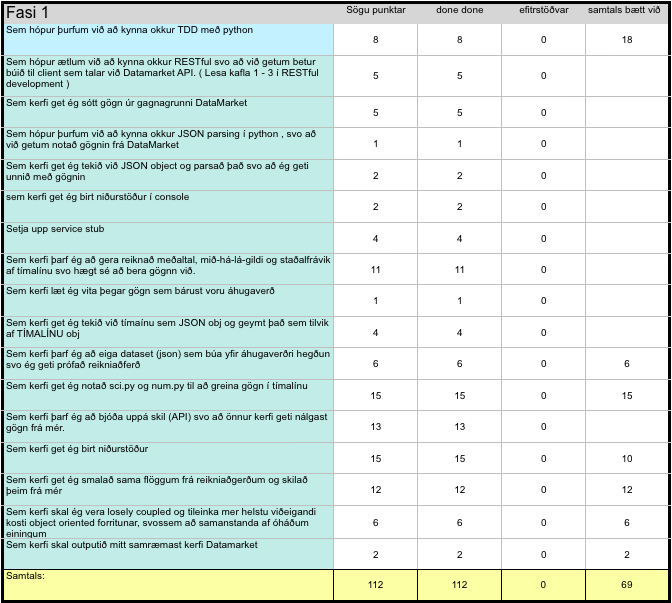
\includegraphics[width=1\textwidth]{Fasi1.png} 
  \caption{Fasi 1} 
\end{figure}

\begin{figure}[H]
  \centering
  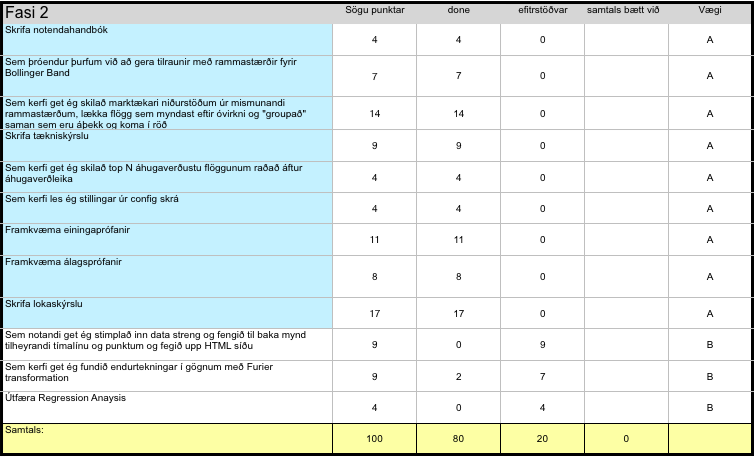
\includegraphics[width=1\textwidth]{Fasi2.png} 
  \caption{Fasi 2} 
\end{figure}

\newpage

\subsection{Burndown}
Hér ber að líta burndown rit yfir framvindu verkefnisins.

\begin{figure}[H]
  \centering
  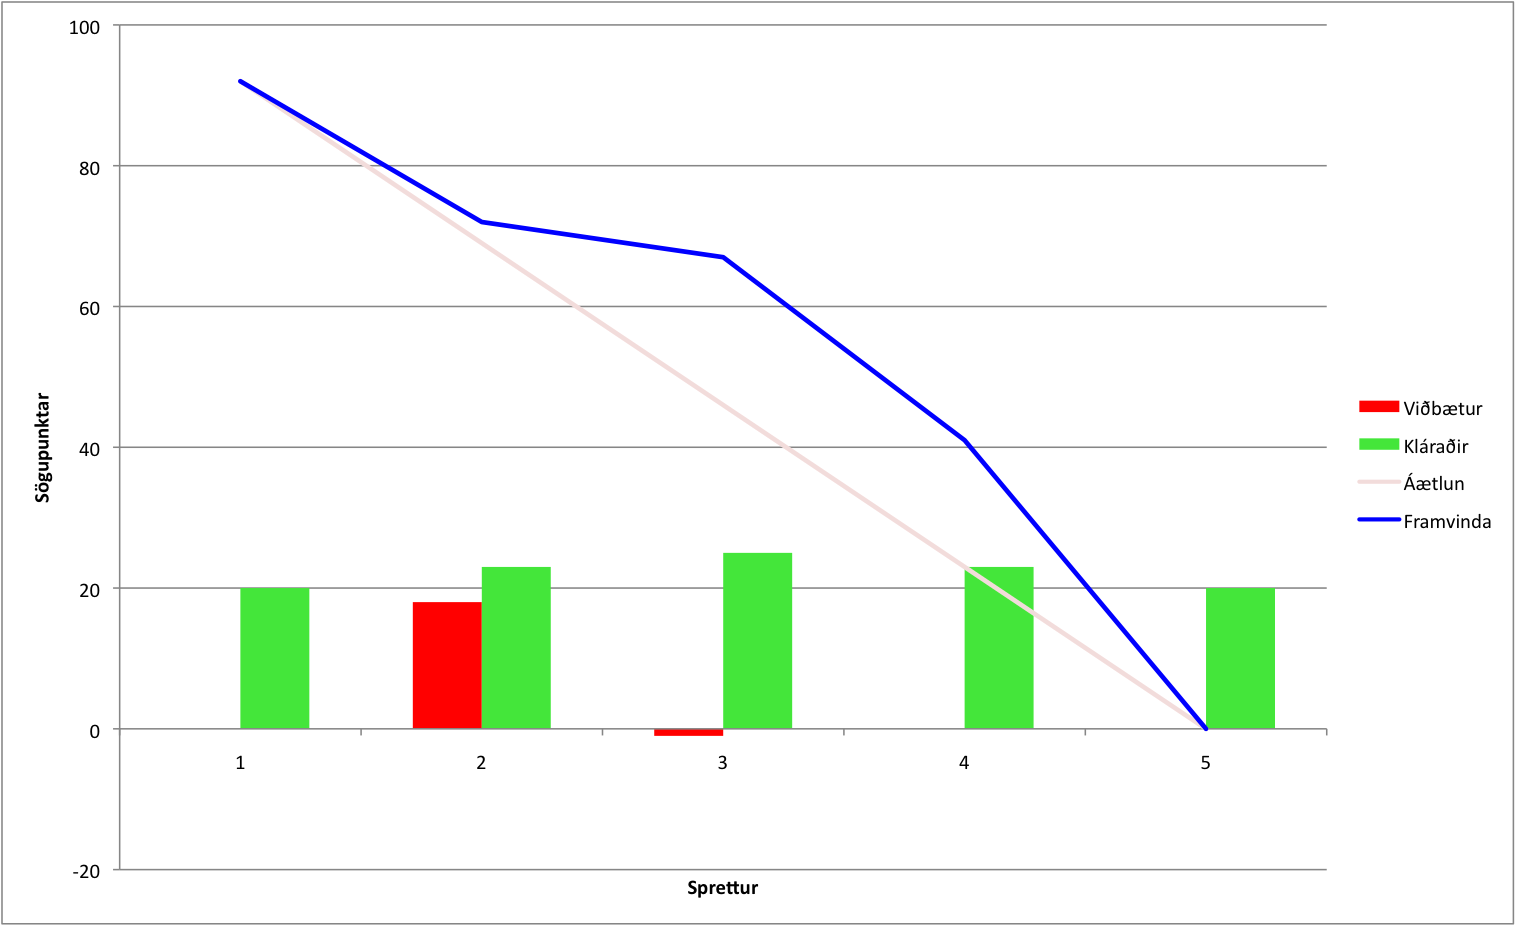
\includegraphics[width=0.8\textwidth]{Fasi1_burndown.png} 
  \caption{Fasi 1} 
\end{figure}

\begin{figure}[H]
  \centering
  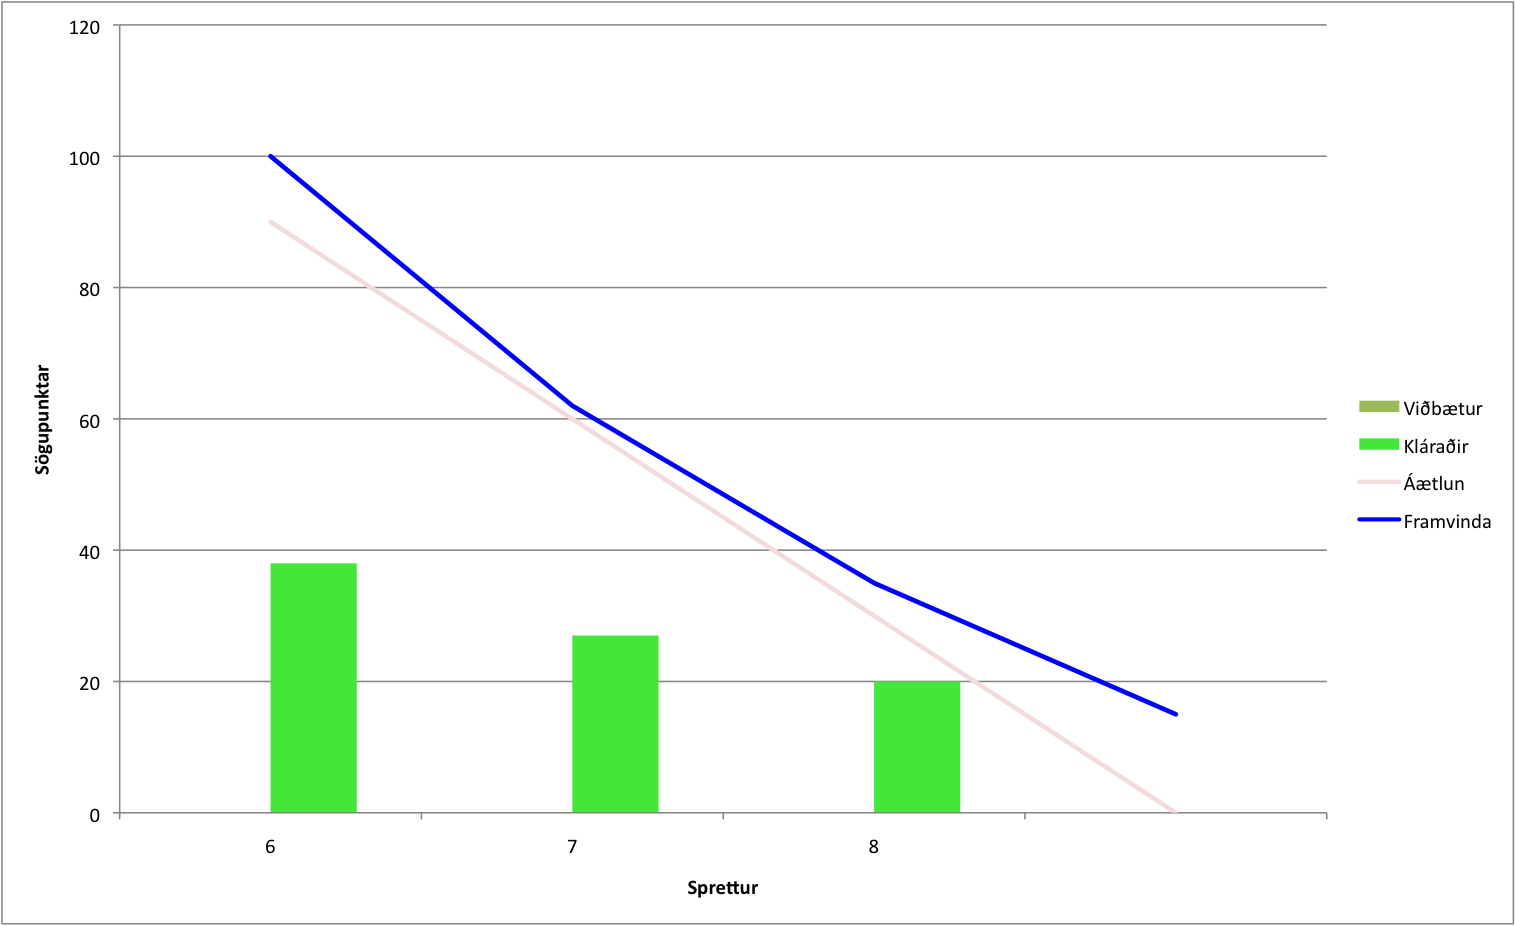
\includegraphics[width=0.8\textwidth]{Fasi2_burndown.png} 
  \caption{Fasi 2} 
\end{figure}

\newpage
\section{Sprettir}
Hér má sjá burndown gröf fyrir spretti verkefnisins. Hægt að er sjá sögur 
hvers spretts fyrir sig í meðfylgjandi skjali Sprettir.pdf. Þar er einnig 
hægt að sjá verkliði fram að sprett 7 en þá var rafrænni skráningu þeirra 
hætt. Var það gert þar sem ekki var þörf á henni lengur vegna þess að við vorum allir saman 
alla daga í vinnuaðstöðunni okkar og höfðum scrum-veggin í augsýn.

\subsection{Sprettur 1}

\begin{figure}[H]
  \centering
  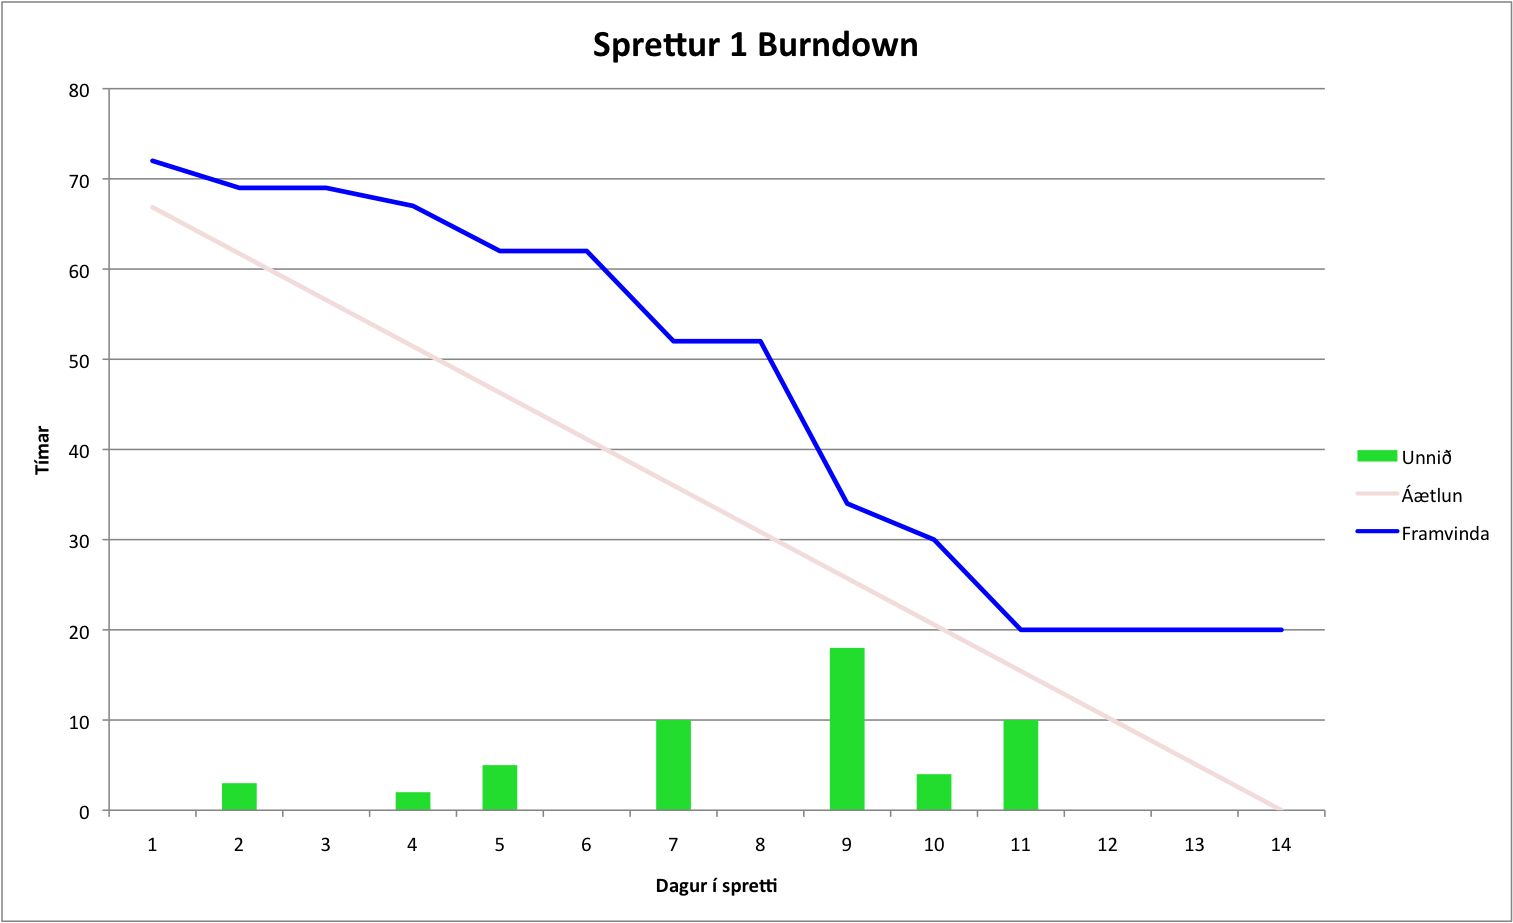
\includegraphics[width=0.8\textwidth]{Sprettur1_Burndown.png} 
  \caption{Sprettur 1} 
\end{figure}

\subsection{Sprettur 2}

\begin{figure}[H]
  \centering
  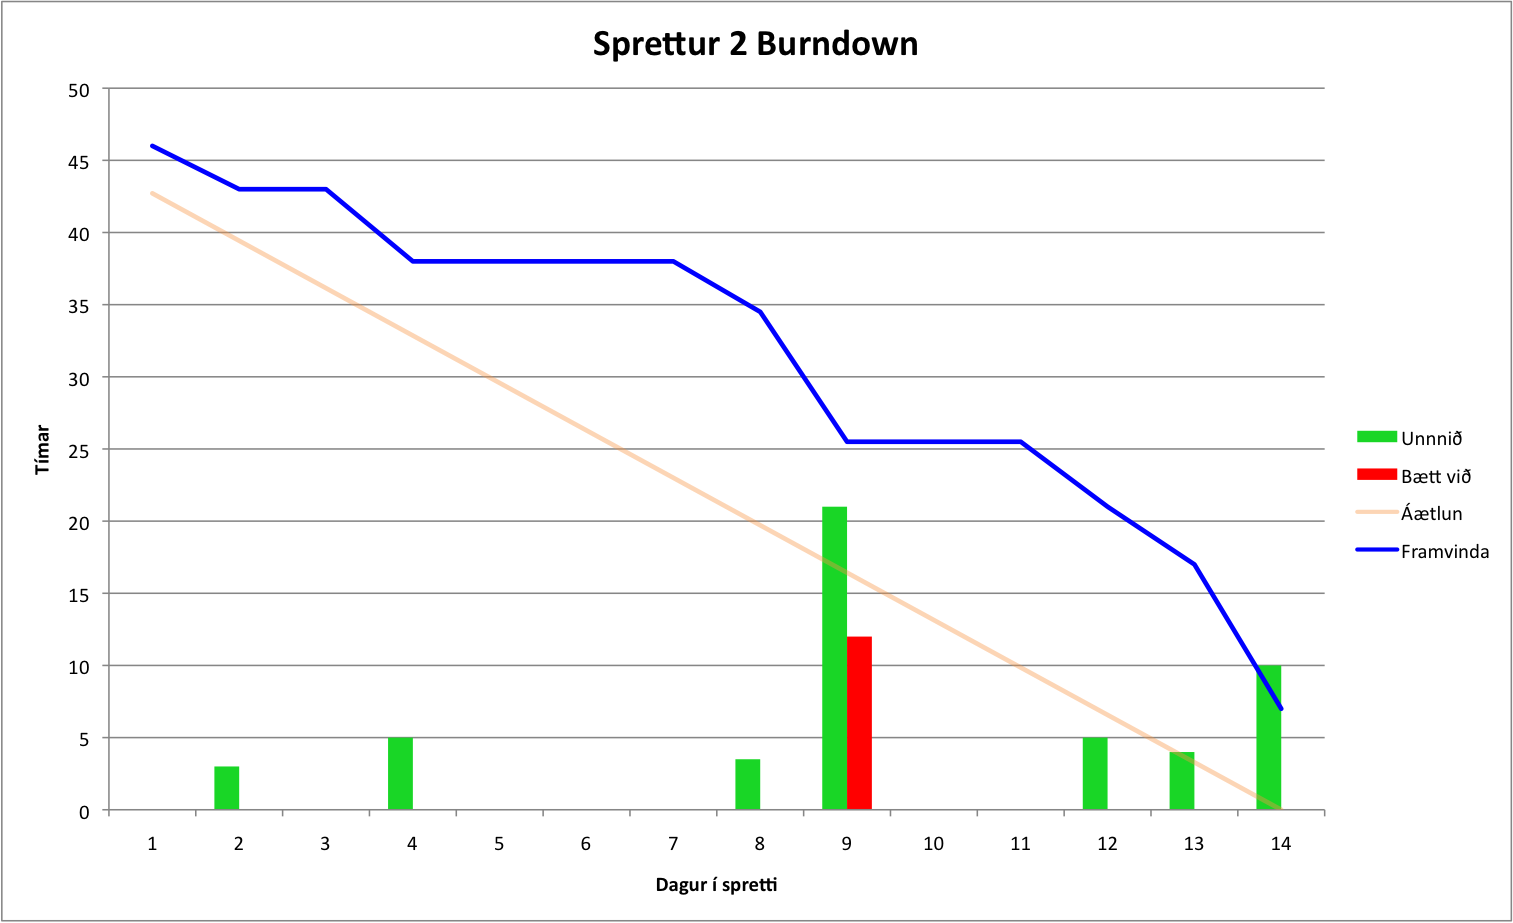
\includegraphics[width=0.8\textwidth]{Sprettur2_Burndown.png} 
  \caption{Sprettur 2} 
\end{figure}

\subsection{Sprettur 3}

\begin{figure}[H]
  \centering
  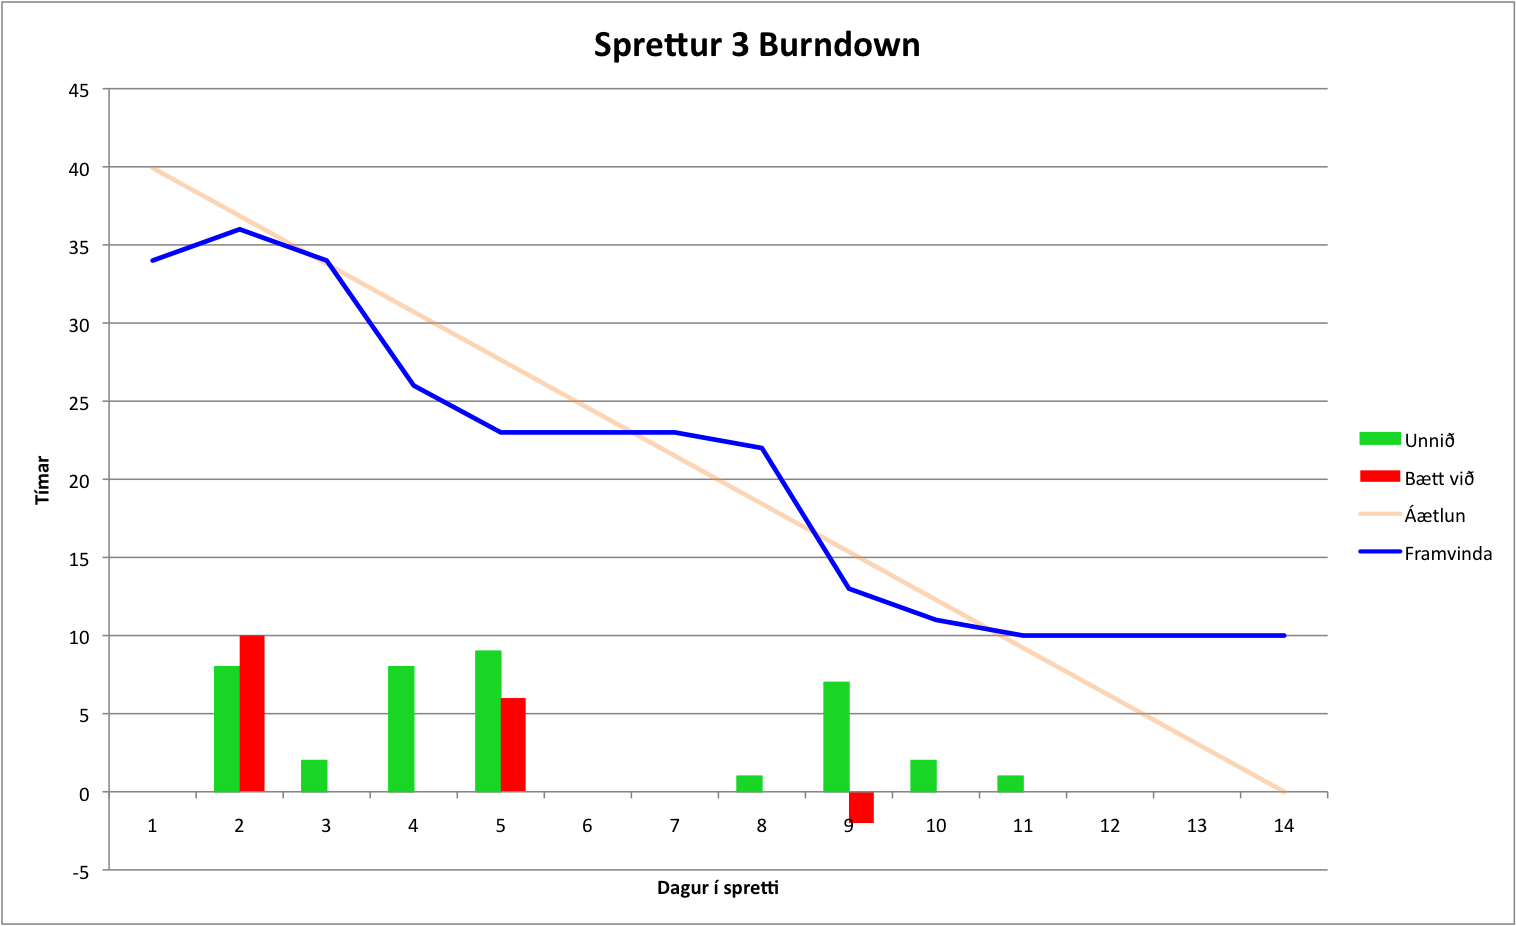
\includegraphics[width=0.8\textwidth]{Sprettur3_Burndown.png} 
  \caption{Sprettur 3} 
\end{figure}

\subsection{Sprettur 4}

\begin{figure}[H]
  \centering
  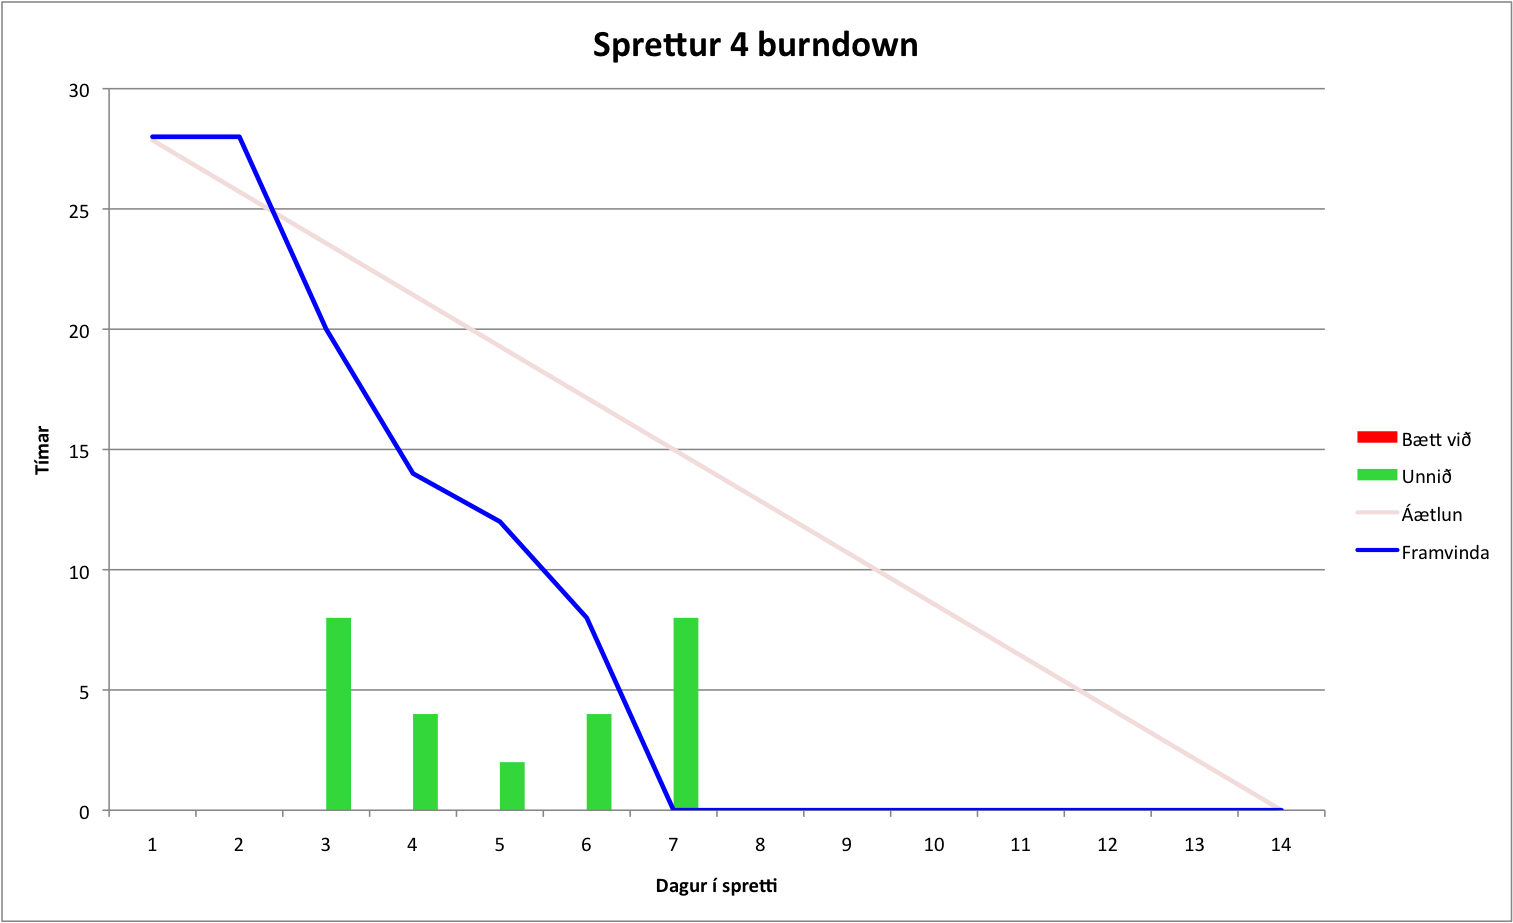
\includegraphics[width=0.8\textwidth]{Sprettur4_Burndown.png} 
  \caption{Sprettur 4} 
\end{figure}

\subsection{Sprettur 5}

\begin{figure}[H]
  \centering
  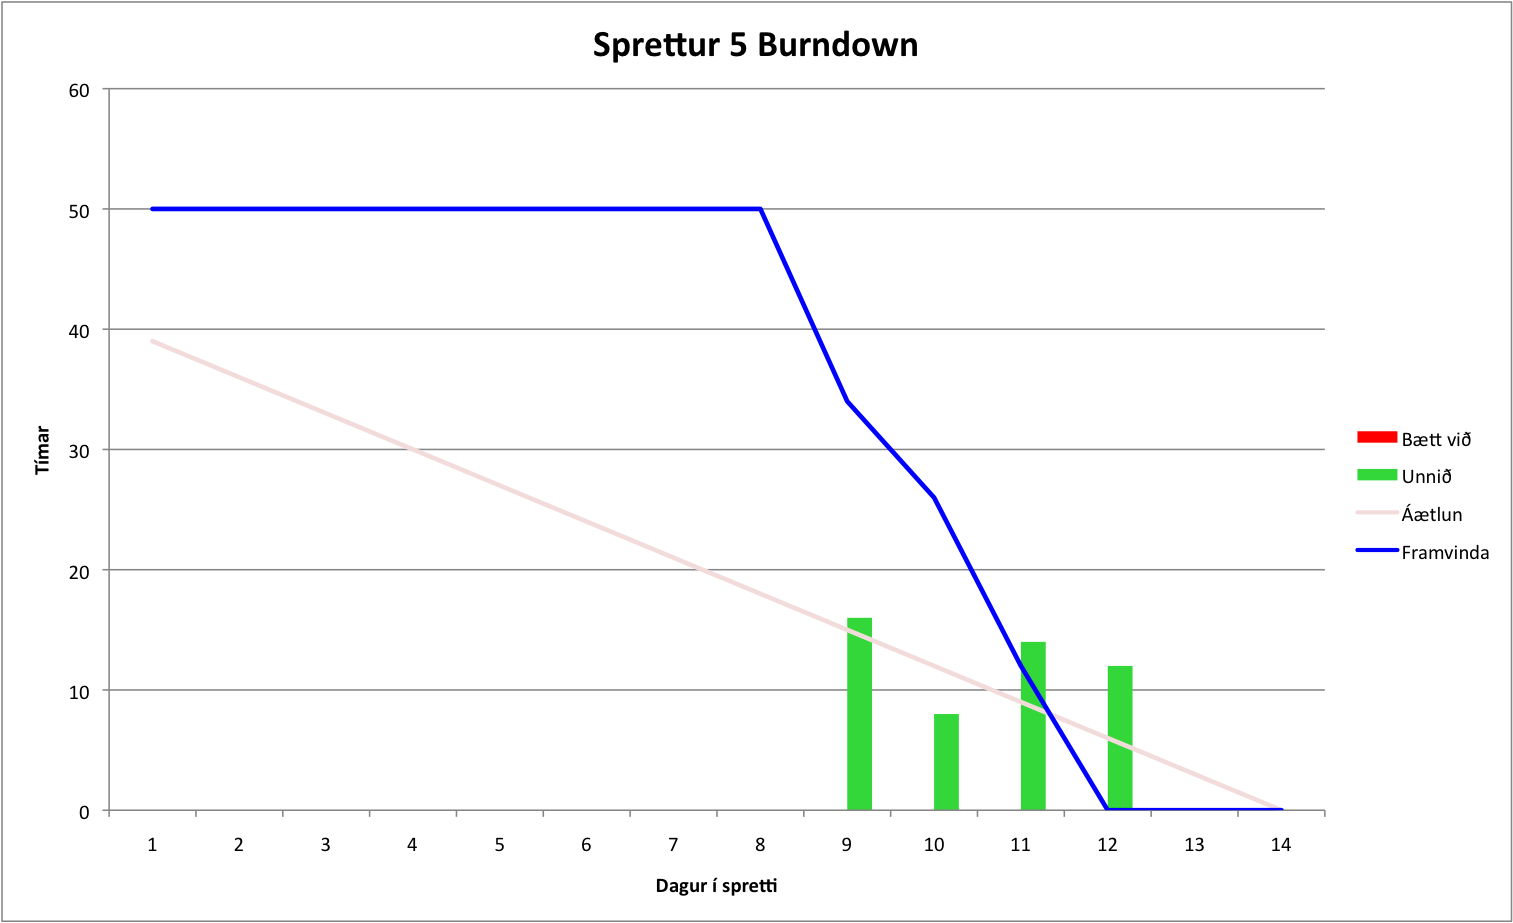
\includegraphics[width=0.8\textwidth]{Sprettur5_Burndown.png} 
  \caption{Sprettur 5} 
\end{figure}

\subsection{Sprettur 6}

\begin{figure}[H]
  \centering
  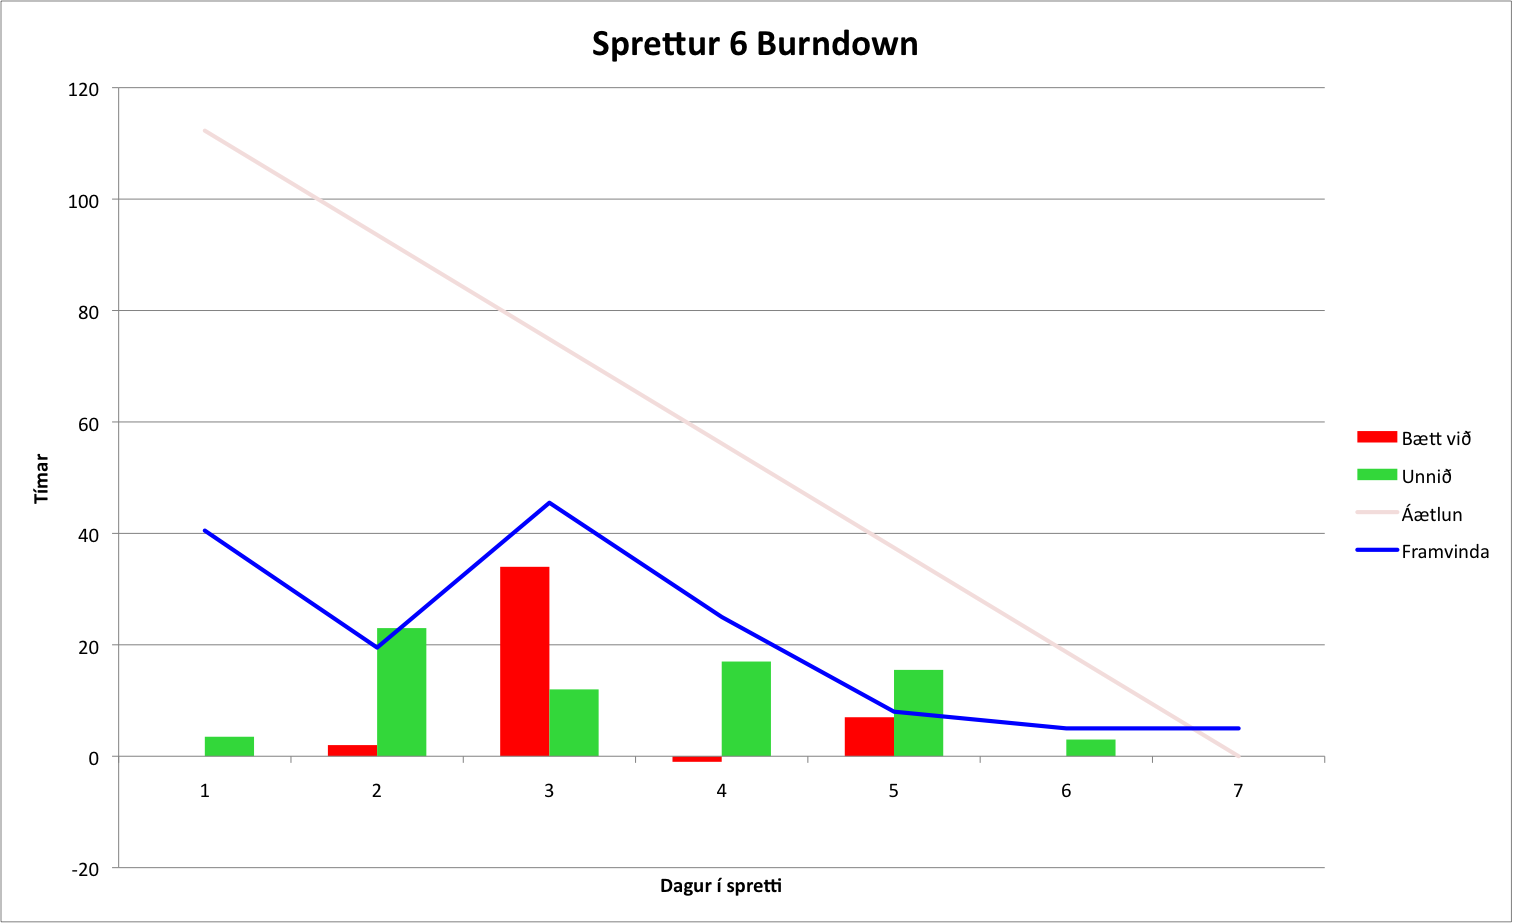
\includegraphics[width=0.8\textwidth]{Sprettur6_Burndown.png} 
  \caption{Sprettur 6} 
\end{figure}

\subsection{Sprettur 6}

\begin{figure}[H]
  \centering
  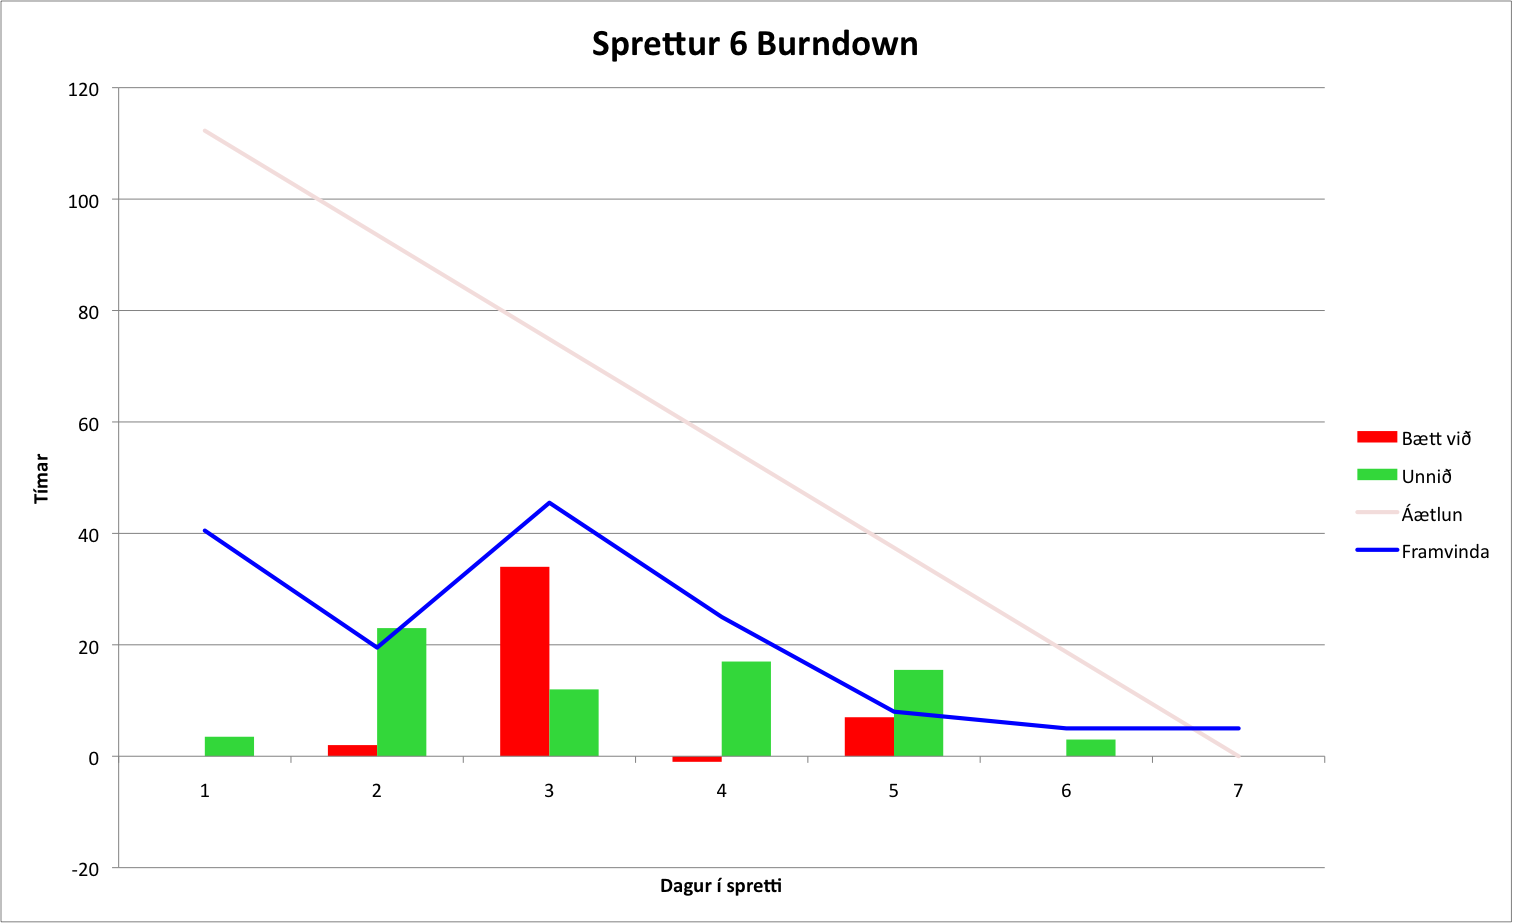
\includegraphics[width=0.8\textwidth]{Sprettur6_Burndown.png} 
  \caption{Sprettur 6} 
\end{figure}

\subsection{Sprettur 7}

\begin{figure}[H]
  \centering
  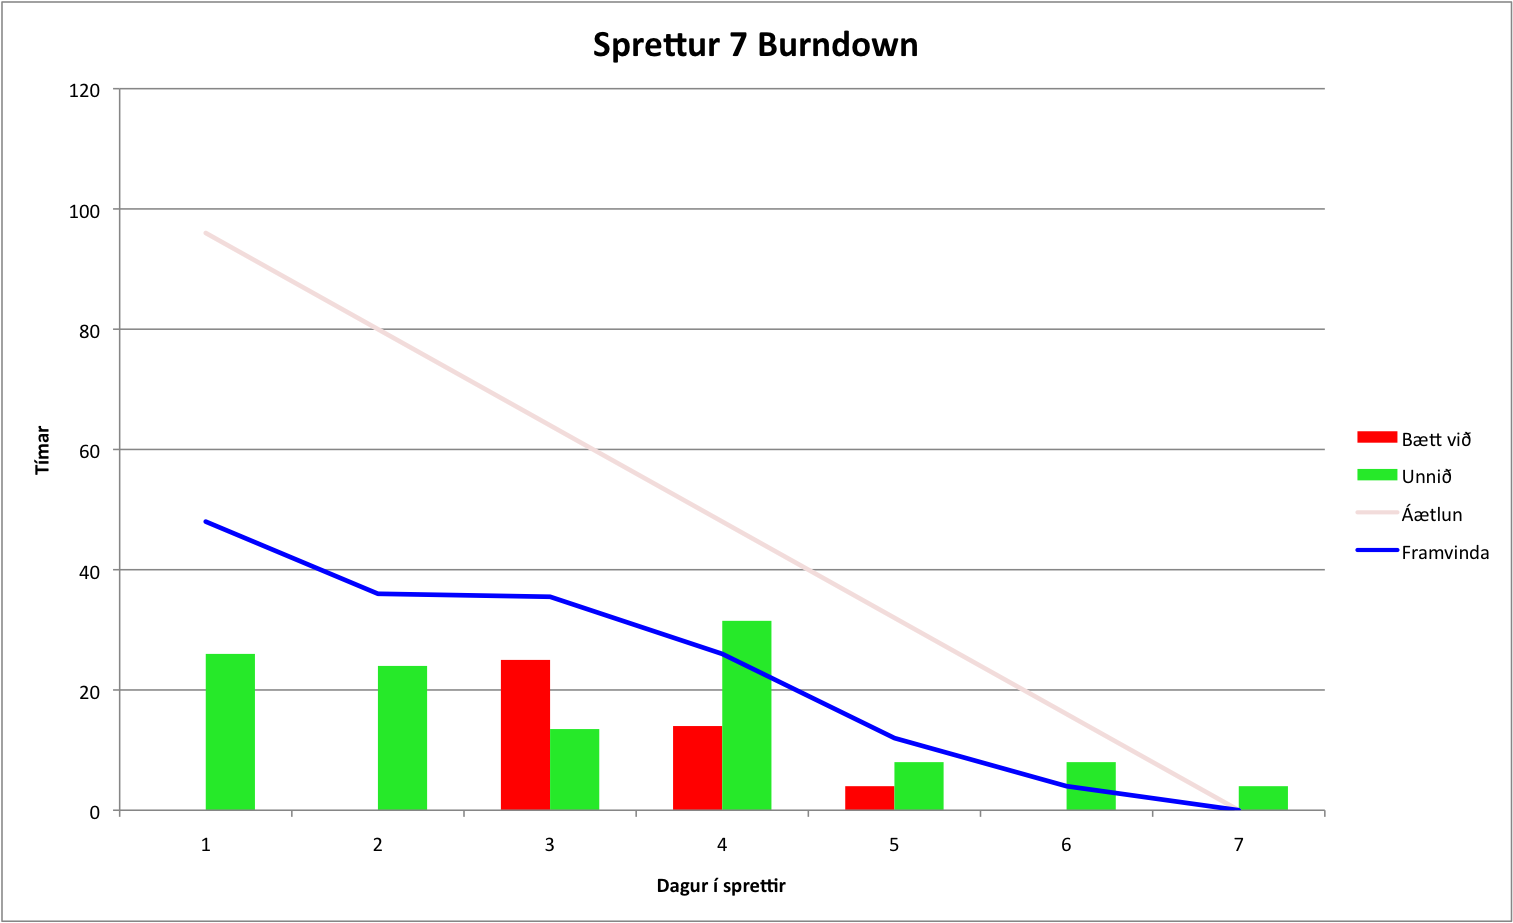
\includegraphics[width=0.8\textwidth]{Sprettur7_Burndown.png} 
  \caption{Sprettur 7} 
\end{figure}

\subsection{Sprettur 8}

\begin{figure}[H]
  \centering
  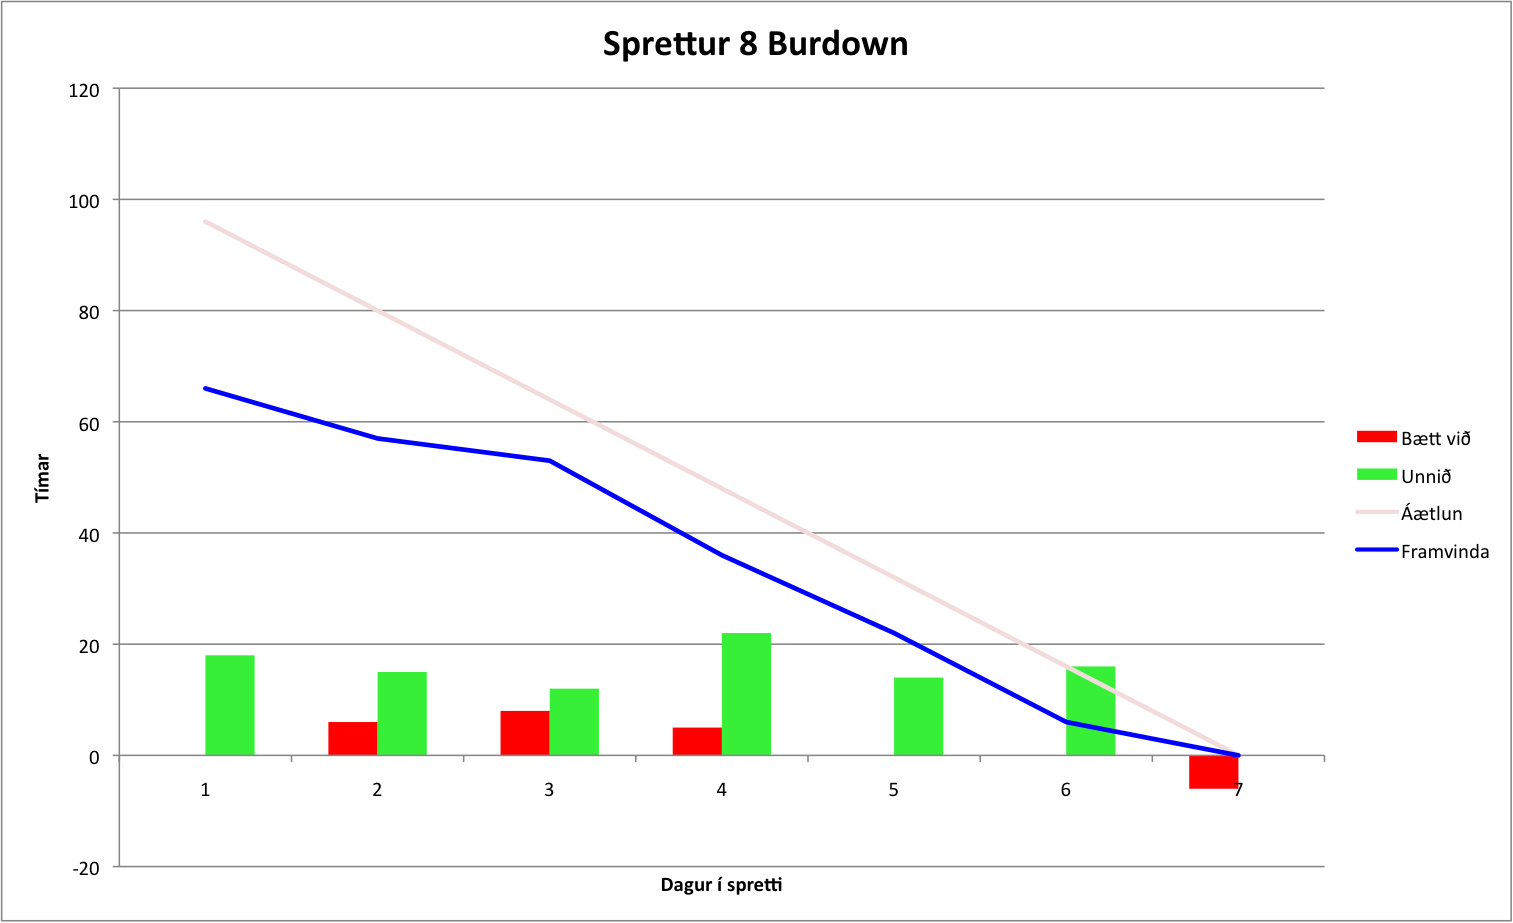
\includegraphics[width=0.8\textwidth]{Sprettur8_Burndown.png} 
  \caption{Sprettur 8} 
\end{figure}

\newpage	
\section{Tímaskráning}
Hér má sjá yfirlit yfir þá tíma sem unnir voru í verkefninu. 

\begin{figure}[H]
  \centering
  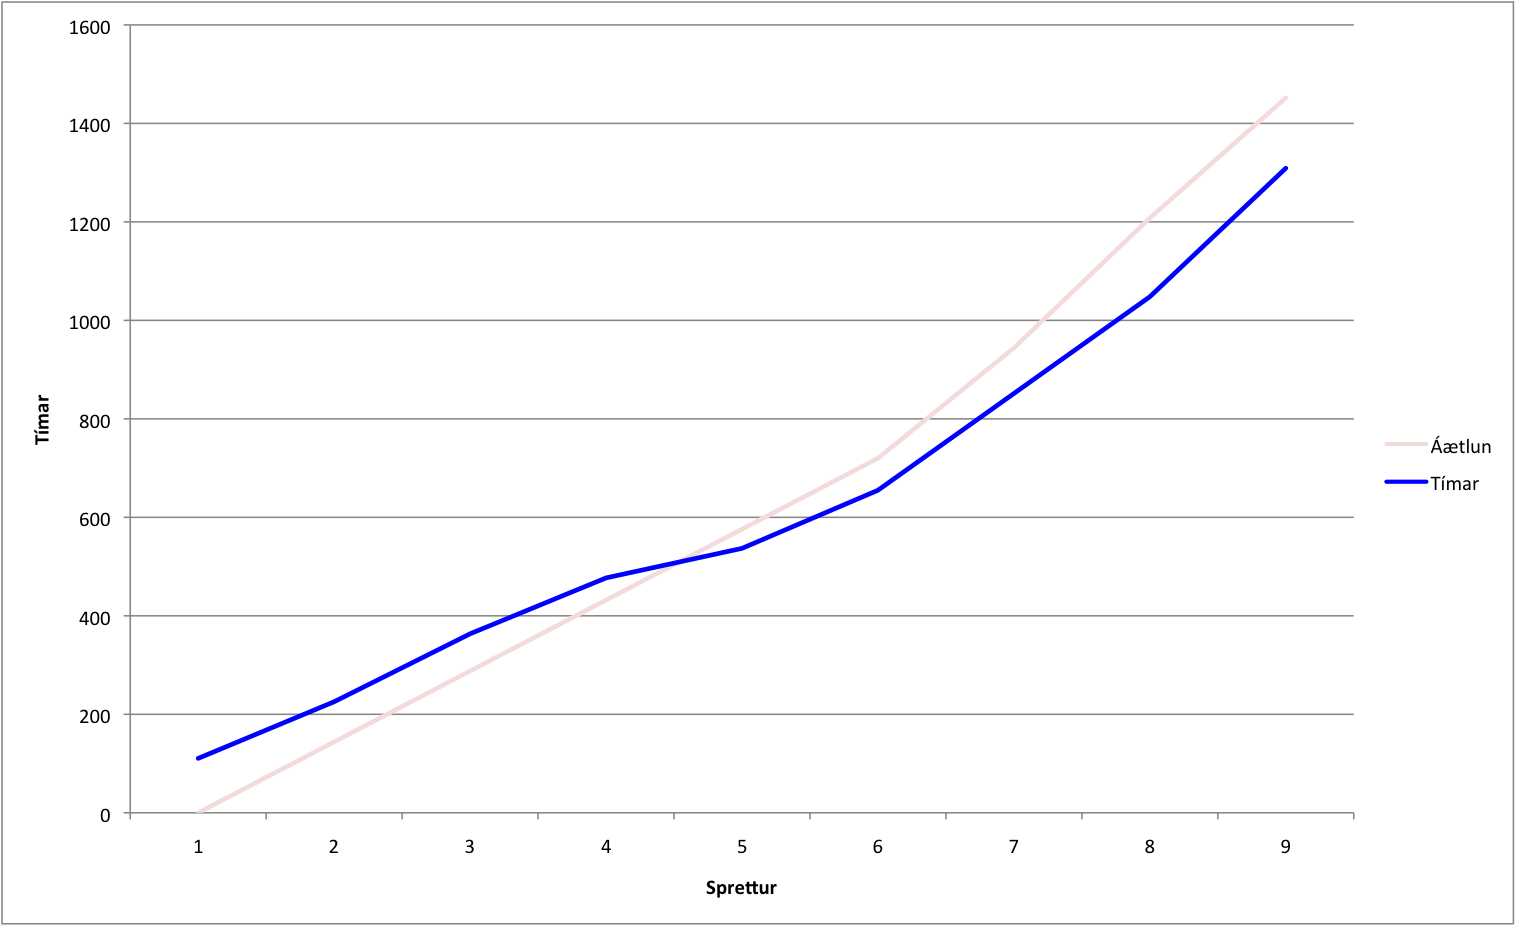
\includegraphics[width=0.8\textwidth]{fjoldi_vinnustunda.png} 
  \caption{fjöldi vinnustunda} 
\end{figure}

Taka ber fram að tímaáætlarnir okkar miðuðust við fyrsta til áttunda sprett og er það 
ástæða þess að tímalínan byrjar ekki á núlli. Í upphafi hennar eru meðtaldir allir tímar 
fram að fyrsta sprett.
Mjög vel gekk að fylgja áætlun að undanskildum sprett 4. Ástæða þess var sú að 
vinna við verkefni í öðrum áföngum undir lok annar og próflestur tók meiri tíma en við gerðum ráð fyrir.
Hægt er að sjá nánari útskýringu á hvernig tíma okkar var varið í skjalinu Dagbok.pdf á meðfylgjandi disk.

\end{document}